

\documentclass[12pt]{article}
\usepackage{fullpage}
\usepackage{graphicx}
\usepackage{amsfonts}
\usepackage{color}
\usepackage{soul}
\pagestyle{plain}
\setlength{\oddsidemargin}{0.5in}
\setlength{\evensidemargin}{0.5in}
\setlength{\textwidth}{6.0in}
\renewcommand{\baselinestretch}{1.2}
\newcommand{\Dsl}{{\not\!\! D}}
\newcommand{\psl}{{\not\! p}}
\usepackage{gensymb}
\usepackage{tikzsymbols}
\usepackage[utf8]{inputenc}
\usepackage{array}
\usepackage{makecell}
\usepackage{hyperref}

\renewcommand\theadalign{bc}
\renewcommand\theadfont{\bfseries}
\renewcommand\theadgape{\Gape[4pt]}
\renewcommand\cellgape{\Gape[4pt]}

%Above are the packages that are needed for most of the reports that you will write
%%%%%%%%%%%%%%%%%%%%%%%%%%%%%%%%%%%%%%%%%%%



\title{Trigonometry One}
\author{Kody Rogers}
\date{\today}
\begin{document}

\maketitle
\thispagestyle{empty}

%Above is title stuff
%%%%%%%%%%%%%%%%%%%%%%%%%%%%%%%%%%%%%%%%%%%%%
\section{Definitions}
\subsection{Main Trig Functions}

Below is the definitions of the three main trigometric functions

$sin(\theta)=\frac{opposite}{hypotenuse}$,
$cos(\theta)=\frac{adjacent}{hypotenuse}$,
$tan(\theta)=\frac{sin(\theta)}{cos(\theta)} = \frac{opposite}{adjacent}$

Now some explanation is needed, and I believe a diagram is best suited to do the explaining.

\begin{figure}[h]
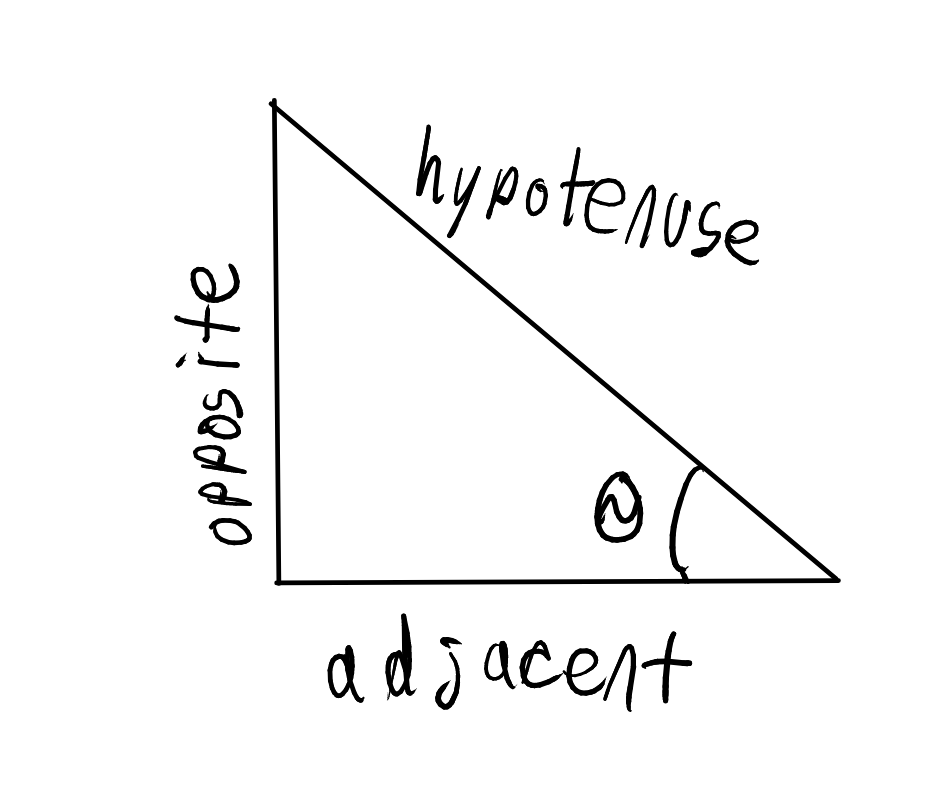
\includegraphics[scale=0.25]{TrigWorksheetTriangle1.png}
\end{figure}

By looking at figure one it can be seen that the hypotenuse is just the side of the right triangle that is largest, and that the opposite side is that opposite to the angle $\theta$ while the adjacent side is the side which the angle sits beside that is not the hypotaneus.

It should be made clear that the formulas so far only work for right triangles.

To get a better feel of these equations let's run through a couple quick examples of them in action.

\subsubsection{Examples}

In the problem below you have to find the side 'B' which happens to be the adjacent side in this picture.
\begin{figure}[h]
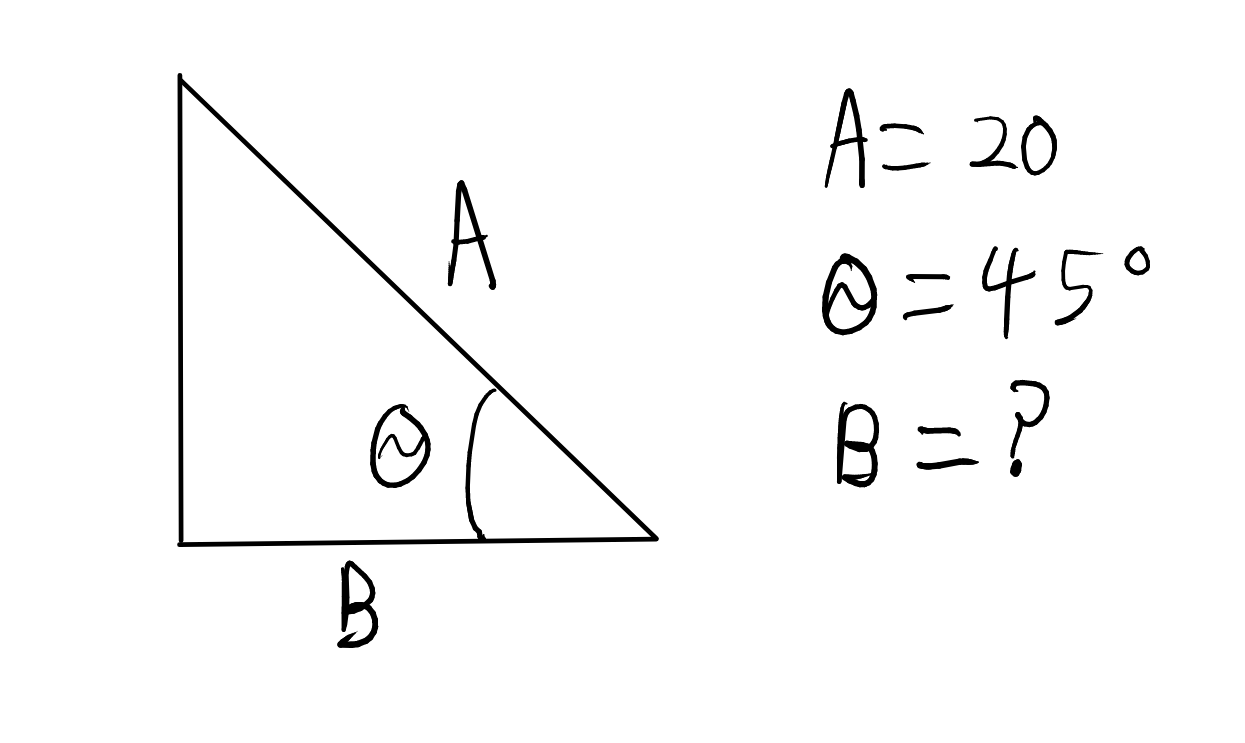
\includegraphics[scale=0.20]{Trigprob1.png}
\end{figure}


\parbox[][12cm][t]{8cm}{}

In the problem below you have to find the 'A' which happens to be the hypotenuse.
\begin{figure}[h]
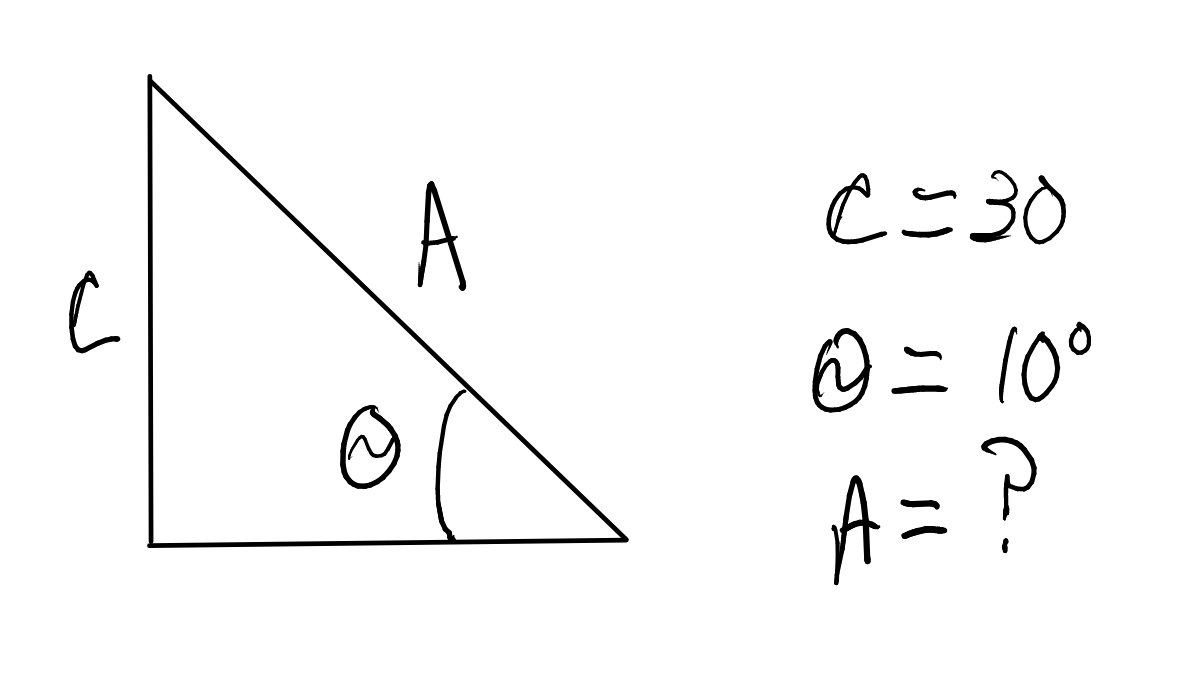
\includegraphics[scale=0.20]{TrigProb2.png}
\end{figure}

\parbox[][5cm][t]{8cm}{}


In the problem below you have to find the 'C' which happens to be the opposite side.
\begin{figure}[h]
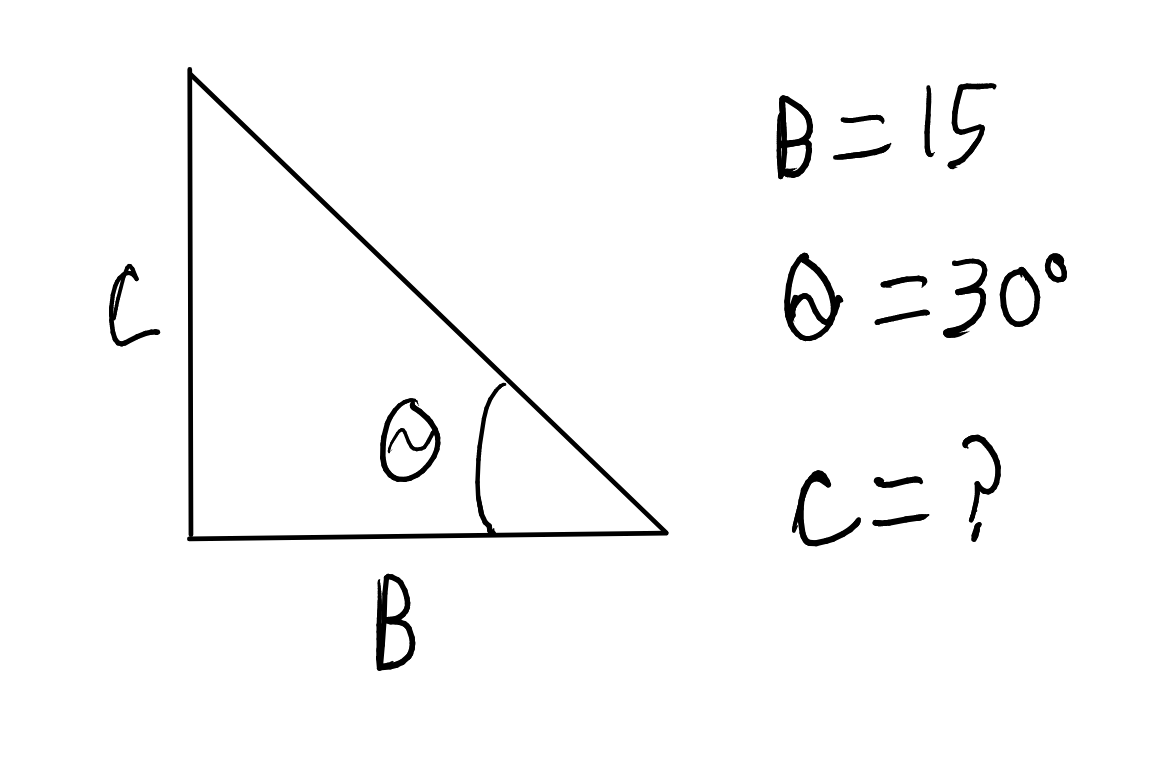
\includegraphics[scale=0.20]{TrigProb3.png}
\end{figure}

\parbox[][2cm][t]{8cm}{}

\subsection{Inverse Trig Functions}

Well it is great that we know how to obtain the side length of right triangles if given one side length and an angle, but what about finding an angle in a right triangle.

One of the angles is 90 degrees and that is what makes it a right triangle, for the others we can use what is called inverse trig functions as long as at least two side lengths are defined.

$sin^{-1}(\frac{opposite}{hypotenuse}) = \theta$,
$cos^{-1}(\frac{adjacent}{hypotenuse}) = \theta$,
$tan^{-1}(\frac{opposite}{adjacent}) = \theta$

Where all the variables are as defined in the first figure.

To be clear the inverse trig function for $sin(\theta)$ is not simply $\frac{1}{sin(\theta)}$ (or any inverse trig function for that matter) which is what one may expect if comparing these inverses to the inverse of a number like '2' which has the inverse of $\frac{1}{2}$. The inverse trig functions undo what the trig functions do, but how that all works is beyond the scope of this workbook.

\subsubsection{Examples}

In the problem below you have to find $\theta$ using the sides 'B' and 'C' or the opposite and adjacent sides.
\begin{figure}[h]
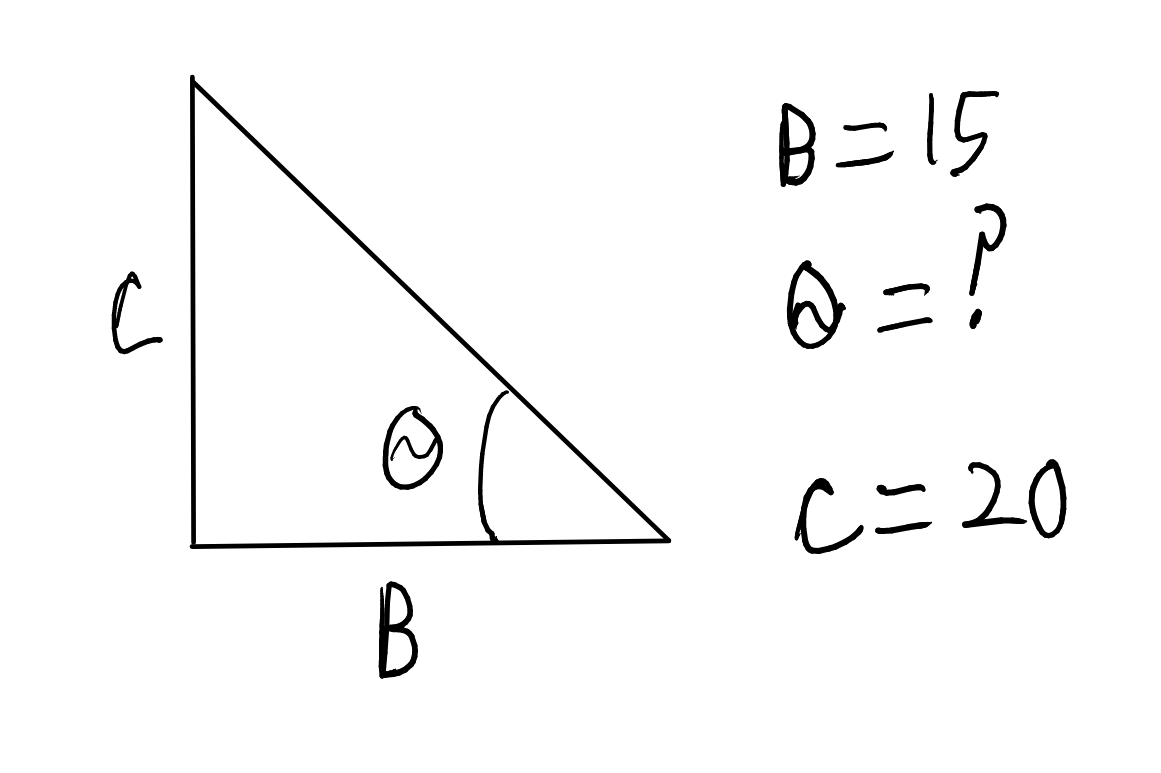
\includegraphics[scale=0.15]{TrigInverseProb1.png}
\end{figure}

\parbox[][6cm][t]{8cm}{}


In the problem below you have to find $\theta$ using the sides 'B' and 'A' or the adjacent and hypotenuse sides.
\begin{figure}[h]
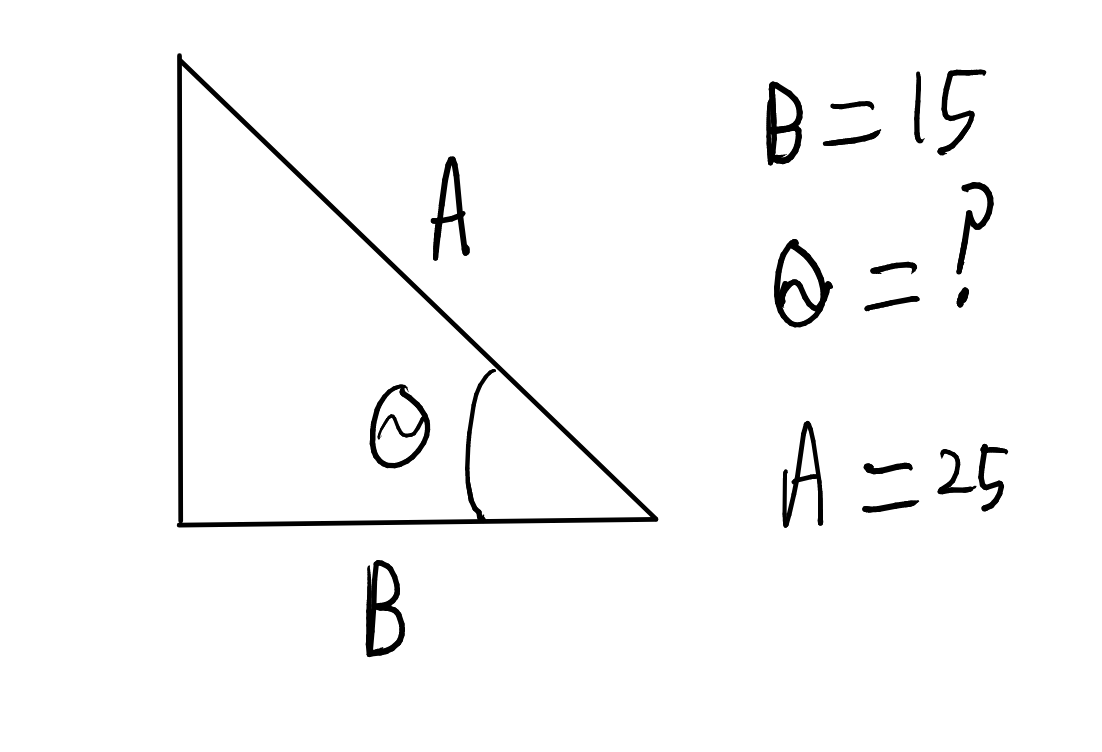
\includegraphics[scale=0.25]{TrigInverseProb2.png}
\end{figure}

\parbox[][13cm][t]{8cm}{}


In the problem below you have to find $\theta$ using the sides 'A' and 'C' or the opposite and hypotenuse sides.
\begin{figure}[h]
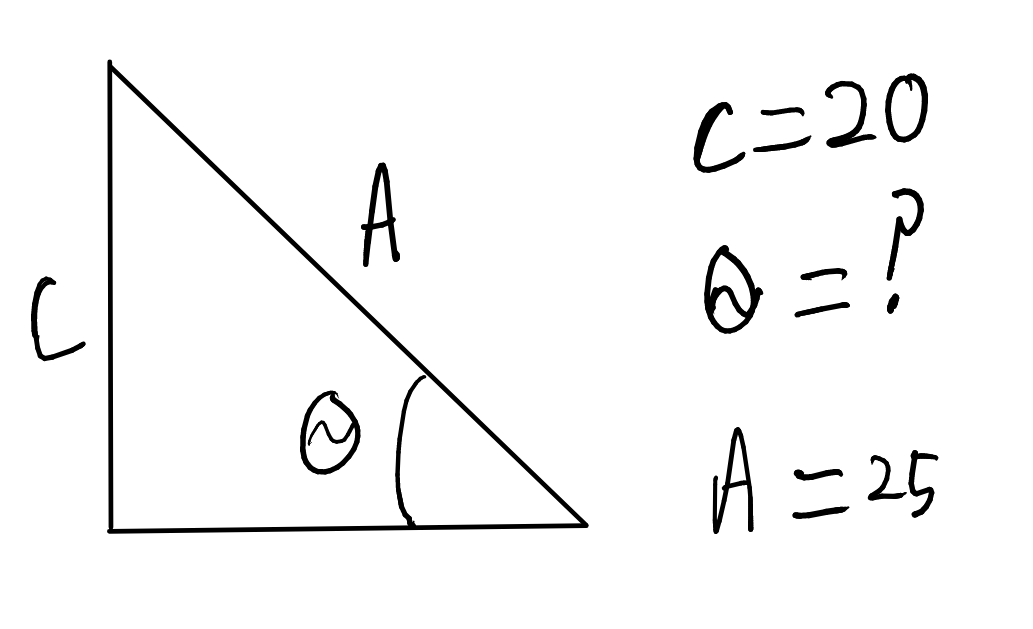
\includegraphics[scale=0.25]{TrigInverseProb3.png}
\end{figure}

\parbox[][8cm][t]{8cm}{}

\section{The Laws of Sine and Cosine}
While it is great that we can find all the sides and angles of a right triangle if we are given two sides, or a side and an angle it would be great to apply these formulas to none right triangles. We can use our current knowledge to derive some formulas that will help us with any triangle. Those formulas are the law of cosine and the law of sine.

\subsection{Law of Sin}
To start with let's write down a arbitrary triangle.

\begin{figure}[h]
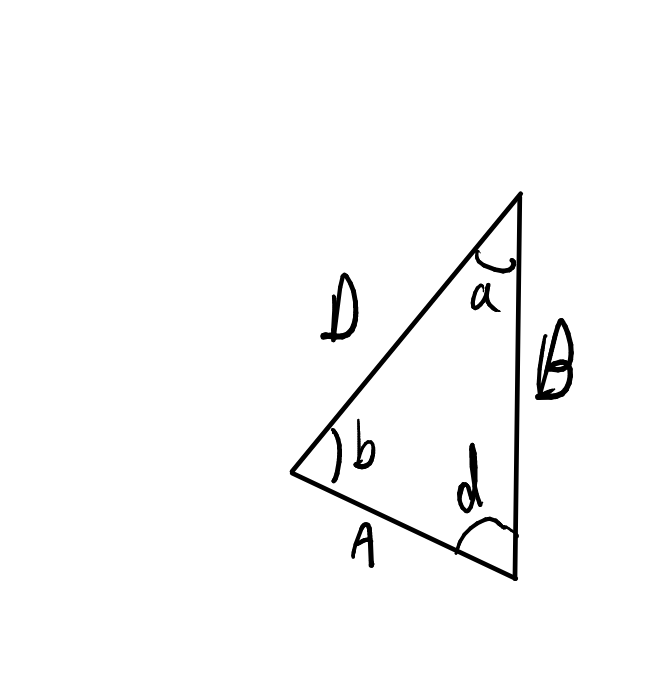
\includegraphics[scale=0.25]{lawOfSin1.png}
\end{figure}

Now I think it would be easier to complete this exercise if the one side of the triangle was horizontally aligned with the words on this page as shown below.

\begin{figure}[h]
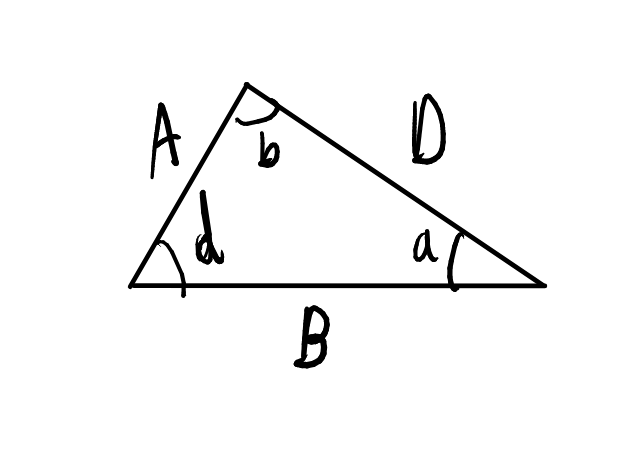
\includegraphics[scale=0.25]{lawOfSin2.png}
\end{figure}

Now the next step is to divide our current triangle into two separate right triangles. I believe you can do this step on your own, so edit the triangle given before moving to the next step.

Now that we have two right triangles we can get an equation involving the angles 'a' and 'd' as well as there corresponding side 'A' and 'D'. After finding that equation it would be useful to have the angle 'a' and the side 'A' on one side of the equation and angle 'd' and side 'D' on the other side of the equation.

\parbox[][5cm][t]{8cm}{}

Now that we have an equation relating the angles 'a' and 'd' along with there corresponding sides it might be useful to find another equation relating the angle 'b' and its corresponding side.

To do this I would go about it the same way as was previously done but putting the side A at the bottom of the triangle instead of side B. I will let you work this out yourself.

\parbox[][12cm][t]{8cm}{}


\subsubsection{Examples}
In the following problem you have to find the side 'B'.
\begin{figure}[h]
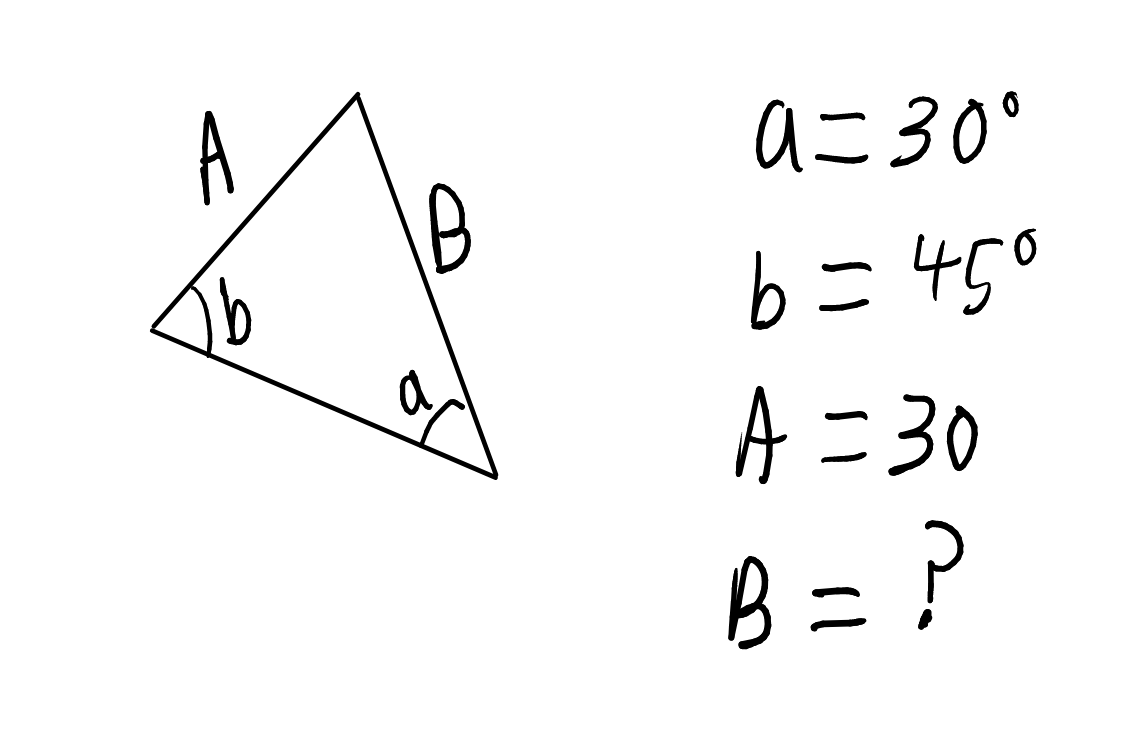
\includegraphics[scale=0.25]{lawOfSinProb1.png}
\end{figure}

\parbox[][13cm][t]{8cm}{Enter your work here}

In the following problem you have to find the angle 'b'.
\begin{figure}[h]
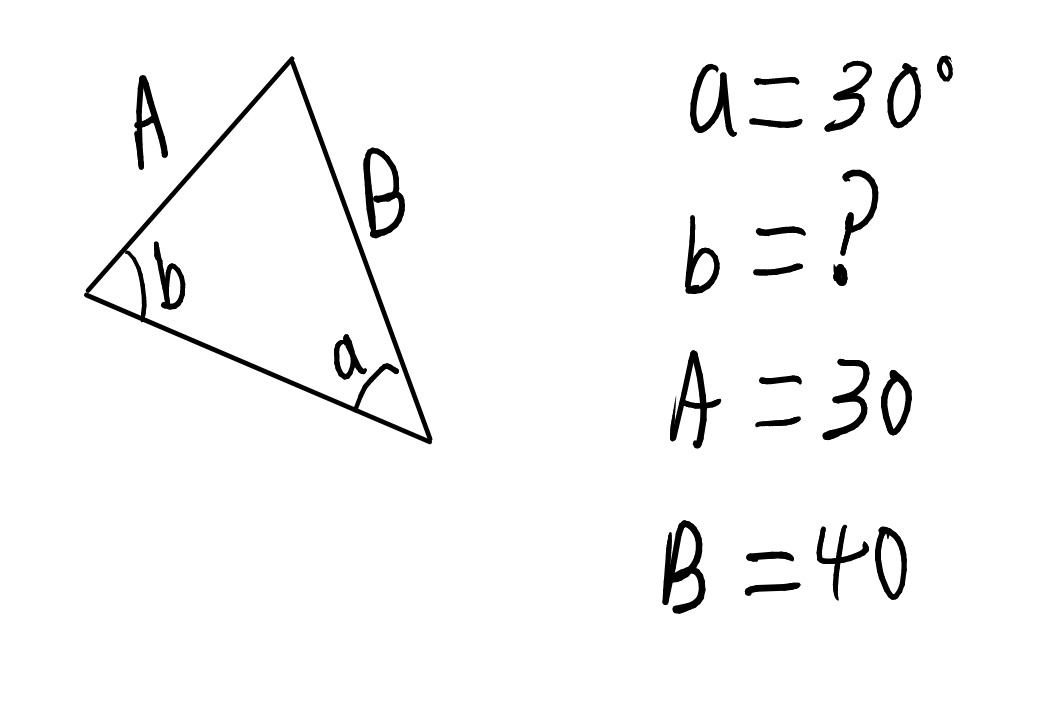
\includegraphics[scale=0.25]{lawOfSinProb2.png}
\end{figure}

\parbox[][8cm][t]{8cm}{}

\subsection{Law of Cosine}

To find the law of cosine we will need the following equations:

$C^2 = A^2 + B^2$

$sin^2(\theta) + cos^2(\theta) = 1$

The first equation is the pythagarean theorem and the second is a trigonometry identity. Later we will derive the second equation but the first equation we will not derive.

To derive the law of cosines we will again start with an arbitrary triangle. We will find side 'C' of this arbitrary triangle.
\begin{figure}[h]
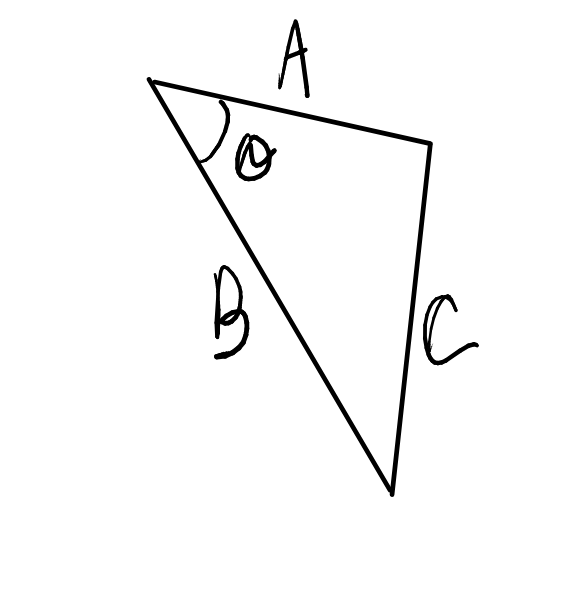
\includegraphics[scale=0.25]{lawOfCosArb.png}
\end{figure}

Now I would again horizontally align this triangle to make the derivation easier, as shown below:
\begin{figure}[h]
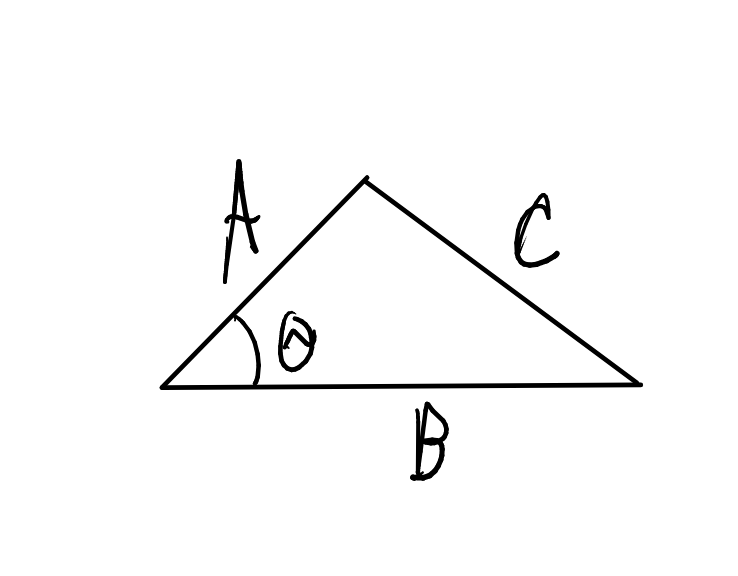
\includegraphics[scale=0.25]{lawOfCosHorizontallyAligned.png}
\end{figure}

The last figure can now be edited in two ways
\begin{enumerate}
  \item By drawing a line down the middle to make two right triangles as done in the derivation of the law of sine.
  \item A third right triangle can be made with side 'C' as the hypotaneus. That triangle is shown below, but I would recommend drawing it on the image above.
\end{enumerate}

\begin{figure}[h]
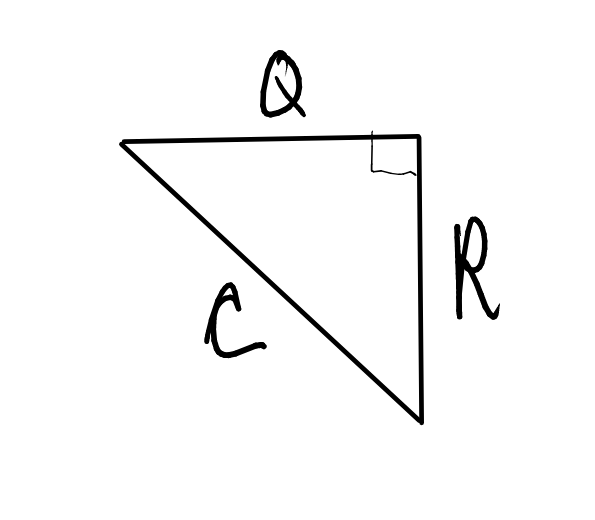
\includegraphics[scale=0.2]{lawOfCosinsQRC2.png}
\end{figure}

The value R can be found by using our knowledge of sin and the values of $\theta$ and 'A'. Write it down below.

\parbox[][4cm][t]{8cm}{}

The value for 'Q' is slightly more complicated but I believe you can do it. For 'Q' the values 'A' and $\theta$ are needed again, but so is 'B'. Write you answer below.

\parbox[][4cm][t]{8cm}{}

Now those two equations can be subsituted into the following equation:

$C^2 = Q^2 + R^2$

And then we have an expression for 'C' with variables and functions that we know.

Sub in these values and find that expression. You will need the formula $sin^2(\theta) + cos^2(\theta) = 1$

\parbox[][8cm][t]{8cm}{}

\section{Trigometric Identities}

Trigometric identities, trig identities for short, are incredibly useful for in math and physics. The most famous trig identity was used in the derivation of the Law of Cosine, and that is one example of its usefulness. In the next section you will derive that famous trig identity. Below I have included a few useful trig identities, but there are many more online.

sin(A $\pm$ B) = sin(A)cos(B) $\pm$ cos(A)sin(B)

cos(A $\pm$ B) = cos(A)cos(B) $\mp$ sin(A)sin(B)

sin(2A) = 2sin(A)cos(A), tan(2A) = $\frac{2tan(A)}{1 - tan^2(A)}$

$cos(2A) = cos^2(A) - sin^2(A) = 1 - 2sin^2(A) = 2cos^2(A) - 1$

If the derivation of these identities are something of interest I would make a worksheet about them :).

\subsection{Most Loved Trig Identity}

We will now derive the most loved trig identity using our knowledge of cosine and sine as well as the pythegarian theorem. That identity is none other than:

$sin^2(\theta) + cos^2(\theta) = 1$

\begin{figure}[h]
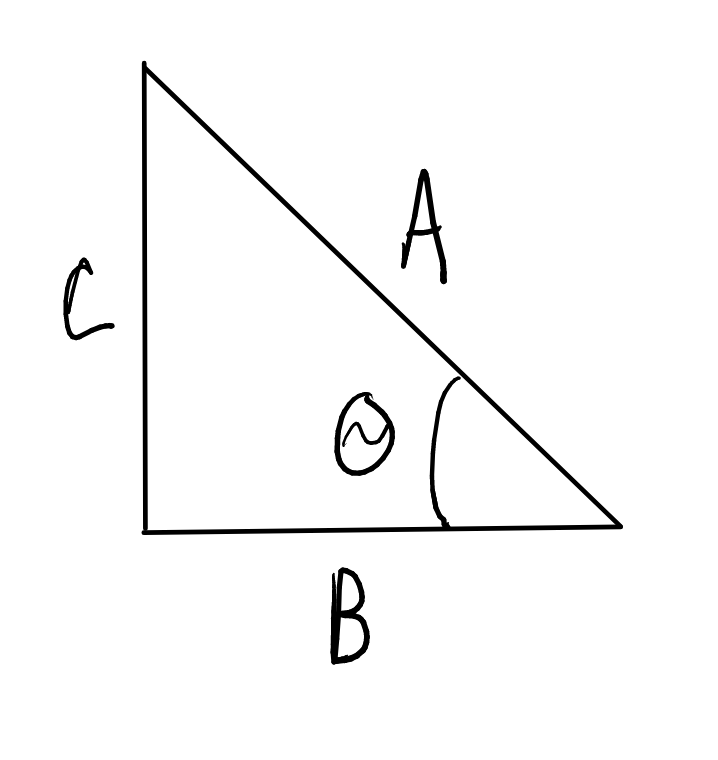
\includegraphics[scale=0.25]{TrigFirstDerivation.png}
\end{figure}

Looking at the triangle write down equations of 'C' and 'B' using the knowledge of sine and cosine covered earlier in the worksheet.

\parbox[][4cm][t]{8cm}{}

With the value of 'C' and 'B' we can find 'A' using the pythegarian theorem. Please write that result below and find the identity that we are looking for.

\parbox[][6cm][t]{8cm}{}

\section{More Interesting Examples}

\subsection{Canon Ball!}
A canon ball is fired at an angle of 45 degrees with respect to the horizontal. The total speed of the canon ball is $25 \frac{km}{s}$. How fast is the canon ball going horizontally?

First I would recommend drawing a picture and then I think the definition fo cosine would be useful.

\parbox[][6cm][t]{8cm}{}


\subsection{Sniper! Sniper!}
A sniper shot a person on a side street 10m away from an office building. The cops arrive at the scene and can tell from the evidence that the bullet came in at an angle of 20 degrees with respect to the ground. If sniper was directly above the victim, but just offset by the 10m separating the victim from the shooter how high up in the office building was the sniper?

First draw a right triangle to deal with this situation. Keep in mind that the adjacent/bottom side is 10m and the opposite side is the height at which the sniper was in the office building

\parbox[][6cm][t]{8cm}{}

Know use your knowledge of trigonometry to find an expression for how high the sniper was:

\parbox[][6cm][t]{8cm}{}

\subsection{Your Closer!}
There are two friends one in Humboldt, Saskatchewan called Dave and the other in Melfort, Saskatchewan called Susan. Dave says that Melfort is closer to Saskatoon than Humboldt is. Dave defends himself by saying that Melfort and Humboldt is 80km apart and Melfort and Saskatoon are 161km apart. Susan says he is wrong, but she suggests to ask their teacher. The teacher says Dave is right about those distances and gives them a hint to the answer by saying the angle between the two sides Dave already stated is 34.2 degrees. The teacher further hints that the law of cosine would give Dave and Susan the answer.

Who is right Dave or Susan? Please put your work below.

\parbox[][6cm][t]{8cm}{}




\begin{flushleft}
    \copyright  2020 Kody Rogers - kodyrogers21@gmail.com.

    This work is is licensed under a Creative Commons Attribution 4.0 International License.

    \url{https://creativecommons.org/licenses/by/4.0/}.
\end{flushleft}

%Above is the Discussion
%%%%%%%%%%%%%%%%%%%%%%%%%%%%%%%%%%%%%%%%%%%%%%%%%%%%%%%
\end{document}
